\documentclass[1p]{elsarticle_modified}
%\bibliographystyle{elsarticle-num}

%\usepackage[colorlinks]{hyperref}
%\usepackage{abbrmath_seonhwa} %\Abb, \Ascr, \Acal ,\Abf, \Afrak
\usepackage{amsfonts}
\usepackage{amssymb}
\usepackage{amsmath}
\usepackage{amsthm}
\usepackage{scalefnt}
\usepackage{amsbsy}
\usepackage{kotex}
\usepackage{caption}
\usepackage{subfig}
\usepackage{color}
\usepackage{graphicx}
\usepackage{xcolor} %% white, black, red, green, blue, cyan, magenta, yellow
\usepackage{float}
\usepackage{setspace}
\usepackage{hyperref}

\usepackage{tikz}
\usetikzlibrary{arrows}

\usepackage{multirow}
\usepackage{array} % fixed length table
\usepackage{hhline}

%%%%%%%%%%%%%%%%%%%%%
\makeatletter
\renewcommand*\env@matrix[1][\arraystretch]{%
	\edef\arraystretch{#1}%
	\hskip -\arraycolsep
	\let\@ifnextchar\new@ifnextchar
	\array{*\c@MaxMatrixCols c}}
\makeatother %https://tex.stackexchange.com/questions/14071/how-can-i-increase-the-line-spacing-in-a-matrix
%%%%%%%%%%%%%%%

\usepackage[normalem]{ulem}

\newcommand{\msout}[1]{\ifmmode\text{\sout{\ensuremath{#1}}}\else\sout{#1}\fi}
%SOURCE: \msout is \stkout macro in https://tex.stackexchange.com/questions/20609/strikeout-in-math-mode

\newcommand{\cancel}[1]{
	\ifmmode
	{\color{red}\msout{#1}}
	\else
	{\color{red}\sout{#1}}
	\fi
}

\newcommand{\add}[1]{
	{\color{blue}\uwave{#1}}
}

\newcommand{\replace}[2]{
	\ifmmode
	{\color{red}\msout{#1}}{\color{blue}\uwave{#2}}
	\else
	{\color{red}\sout{#1}}{\color{blue}\uwave{#2}}
	\fi
}

\newcommand{\Sol}{\mathcal{S}} %segment
\newcommand{\D}{D} %diagram
\newcommand{\A}{\mathcal{A}} %arc


%%%%%%%%%%%%%%%%%%%%%%%%%%%%%5 test

\def\sl{\operatorname{\textup{SL}}(2,\Cbb)}
\def\psl{\operatorname{\textup{PSL}}(2,\Cbb)}
\def\quan{\mkern 1mu \triangleright \mkern 1mu}

\theoremstyle{definition}
\newtheorem{thm}{Theorem}[section]
\newtheorem{prop}[thm]{Proposition}
\newtheorem{lem}[thm]{Lemma}
\newtheorem{ques}[thm]{Question}
\newtheorem{cor}[thm]{Corollary}
\newtheorem{defn}[thm]{Definition}
\newtheorem{exam}[thm]{Example}
\newtheorem{rmk}[thm]{Remark}
\newtheorem{alg}[thm]{Algorithm}

\newcommand{\I}{\sqrt{-1}}
\begin{document}

%\begin{frontmatter}
%
%\title{Boundary parabolic representations of knots up to 8 crossings}
%
%%% Group authors per affiliation:
%\author{Yunhi Cho} 
%\address{Department of Mathematics, University of Seoul, Seoul, Korea}
%\ead{yhcho@uos.ac.kr}
%
%
%\author{Seonhwa Kim} %\fnref{s_kim}}
%\address{Center for Geometry and Physics, Institute for Basic Science, Pohang, 37673, Korea}
%\ead{ryeona17@ibs.re.kr}
%
%\author{Hyuk Kim}
%\address{Department of Mathematical Sciences, Seoul National University, Seoul 08826, Korea}
%\ead{hyukkim@snu.ac.kr}
%
%\author{Seokbeom Yoon}
%\address{Department of Mathematical Sciences, Seoul National University, Seoul, 08826,  Korea}
%\ead{sbyoon15@snu.ac.kr}
%
%\begin{abstract}
%We find all boundary parabolic representation of knots up to 8 crossings.
%
%\end{abstract}
%\begin{keyword}
%    \MSC[2010] 57M25 
%\end{keyword}
%
%\end{frontmatter}

%\linenumbers
%\tableofcontents
%
\newcommand\colored[1]{\textcolor{white}{\rule[-0.35ex]{0.8em}{1.4ex}}\kern-0.8em\color{red} #1}%
%\newcommand\colored[1]{\textcolor{white}{ #1}\kern-2.17ex	\textcolor{white}{ #1}\kern-1.81ex	\textcolor{white}{ #1}\kern-2.15ex\color{red}#1	}

{\Large $\underline{12n_{0654}~(K12n_{0654})}$}

\setlength{\tabcolsep}{10pt}
\renewcommand{\arraystretch}{1.6}
\vspace{1cm}\begin{tabular}{m{100pt}>{\centering\arraybackslash}m{274pt}}
\multirow{5}{120pt}{
	\centering
	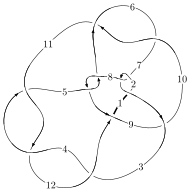
\includegraphics[width=112pt]{../../../GIT/diagram.site/Diagrams/png/2743_12n_0654.png}\\
\ \ \ A knot diagram\footnotemark}&
\allowdisplaybreaks
\textbf{Linearized knot diagam} \\
\cline{2-2}
 &
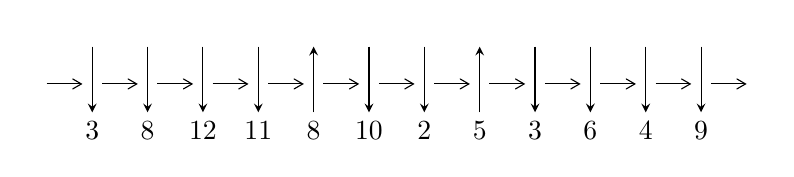
\begin{tikzpicture}[x=20pt, y=17pt]
	% nodes
	\node (C0) at (0, 0) {};
	\node (C1) at (1, 0) {};
	\node (C1U) at (1, +1) {};
	\node (C1D) at (1, -1) {3};

	\node (C2) at (2, 0) {};
	\node (C2U) at (2, +1) {};
	\node (C2D) at (2, -1) {8};

	\node (C3) at (3, 0) {};
	\node (C3U) at (3, +1) {};
	\node (C3D) at (3, -1) {12};

	\node (C4) at (4, 0) {};
	\node (C4U) at (4, +1) {};
	\node (C4D) at (4, -1) {11};

	\node (C5) at (5, 0) {};
	\node (C5U) at (5, +1) {};
	\node (C5D) at (5, -1) {8};

	\node (C6) at (6, 0) {};
	\node (C6U) at (6, +1) {};
	\node (C6D) at (6, -1) {10};

	\node (C7) at (7, 0) {};
	\node (C7U) at (7, +1) {};
	\node (C7D) at (7, -1) {2};

	\node (C8) at (8, 0) {};
	\node (C8U) at (8, +1) {};
	\node (C8D) at (8, -1) {5};

	\node (C9) at (9, 0) {};
	\node (C9U) at (9, +1) {};
	\node (C9D) at (9, -1) {3};

	\node (C10) at (10, 0) {};
	\node (C10U) at (10, +1) {};
	\node (C10D) at (10, -1) {6};

	\node (C11) at (11, 0) {};
	\node (C11U) at (11, +1) {};
	\node (C11D) at (11, -1) {4};

	\node (C12) at (12, 0) {};
	\node (C12U) at (12, +1) {};
	\node (C12D) at (12, -1) {9};
	\node (C13) at (13, 0) {};

	% arrows
	\draw[->,>={angle 60}]
	(C0) edge (C1) (C1) edge (C2) (C2) edge (C3) (C3) edge (C4) (C4) edge (C5) (C5) edge (C6) (C6) edge (C7) (C7) edge (C8) (C8) edge (C9) (C9) edge (C10) (C10) edge (C11) (C11) edge (C12) (C12) edge (C13) ;	\draw[->,>=stealth]
	(C1U) edge (C1D) (C2U) edge (C2D) (C3U) edge (C3D) (C4U) edge (C4D) (C5D) edge (C5U) (C6U) edge (C6D) (C7U) edge (C7D) (C8D) edge (C8U) (C9U) edge (C9D) (C10U) edge (C10D) (C11U) edge (C11D) (C12U) edge (C12D) ;
	\end{tikzpicture} \\
\hhline{~~} \\& 
\textbf{Solving Sequence} \\ \cline{2-2} 
 &
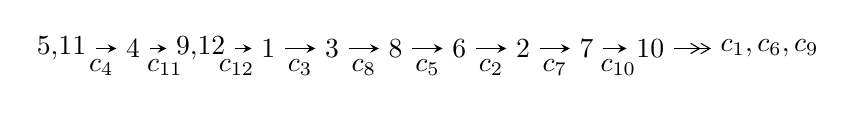
\begin{tikzpicture}[x=23pt, y=7pt]
	% node
	\node (A0) at (-1/8, 0) {5,11};
	\node (A1) at (1, 0) {4};
	\node (A2) at (33/16, 0) {9,12};
	\node (A3) at (25/8, 0) {1};
	\node (A4) at (33/8, 0) {3};
	\node (A5) at (41/8, 0) {8};
	\node (A6) at (49/8, 0) {6};
	\node (A7) at (57/8, 0) {2};
	\node (A8) at (65/8, 0) {7};
	\node (A9) at (73/8, 0) {10};
	\node (C1) at (1/2, -1) {$c_{4}$};
	\node (C2) at (3/2, -1) {$c_{11}$};
	\node (C3) at (21/8, -1) {$c_{12}$};
	\node (C4) at (29/8, -1) {$c_{3}$};
	\node (C5) at (37/8, -1) {$c_{8}$};
	\node (C6) at (45/8, -1) {$c_{5}$};
	\node (C7) at (53/8, -1) {$c_{2}$};
	\node (C8) at (61/8, -1) {$c_{7}$};
	\node (C9) at (69/8, -1) {$c_{10}$};
	\node (A10) at (11, 0) {$c_{1},c_{6},c_{9}$};

	% edge
	\draw[->,>=stealth]	
	(A0) edge (A1) (A1) edge (A2) (A2) edge (A3) (A3) edge (A4) (A4) edge (A5) (A5) edge (A6) (A6) edge (A7) (A7) edge (A8) (A8) edge (A9) ;
	\draw[->>,>={angle 60}]	
	(A9) edge (A10);
\end{tikzpicture} \\ 

\end{tabular} \\

\footnotetext{
The image of knot diagram is generated by the software ``\textbf{Draw programme}" developed by Andrew Bartholomew(\url{http://www.layer8.co.uk/maths/draw/index.htm\#Running-draw}), where we modified some parts for our purpose(\url{https://github.com/CATsTAILs/LinksPainter}).
}\phantom \\ \newline 
\centering \textbf{Ideals for irreducible components\footnotemark of $X_{\text{par}}$} 
 
\begin{align*}
I^u_{1}&=\langle 
u^{18}-5 u^{17}+\cdots+b-7,\;-5 u^{18}+23 u^{17}+\cdots+2 a+19,\;u^{19}-5 u^{18}+\cdots-11 u+2\rangle \\
I^u_{2}&=\langle 
- u^8- u^7-6 u^6-5 u^5-11 u^4-7 u^3-6 u^2+b-2 u,\\
\phantom{I^u_{2}}&\phantom{= \langle  }- u^8-2 u^7-7 u^6-11 u^5-16 u^4-18 u^3-13 u^2+a-8 u-2,\\
\phantom{I^u_{2}}&\phantom{= \langle  }u^{11}+2 u^{10}+9 u^9+14 u^8+29 u^7+34 u^6+40 u^5+32 u^4+20 u^3+7 u^2-1\rangle \\
I^u_{3}&=\langle 
u^2 a- a u+3 u^2+4 b- a+u+5,\;- u^2 a+a^2- a u- u^2-2 a-2 u-4,\;u^3+2 u-1\rangle \\
I^u_{4}&=\langle 
- u^3 a- u^3-2 a u- u^2+b- a-2 u-1,\;- u^3 a+u^3+a^2+2 u^2+a+2 u,\;u^4+u^3+2 u^2+2 u+1\rangle \\
\\
\end{align*}
\raggedright * 4 irreducible components of $\dim_{\mathbb{C}}=0$, with total 44 representations.\\
\footnotetext{All coefficients of polynomials are rational numbers. But the coefficients are sometimes approximated in decimal forms when there is not enough margin.}
\newpage
\renewcommand{\arraystretch}{1}
\centering \section*{I. $I^u_{1}= \langle u^{18}-5 u^{17}+\cdots+b-7,\;-5 u^{18}+23 u^{17}+\cdots+2 a+19,\;u^{19}-5 u^{18}+\cdots-11 u+2 \rangle$}
\flushleft \textbf{(i) Arc colorings}\\
\begin{tabular}{m{7pt} m{180pt} m{7pt} m{180pt} }
\flushright $a_{5}=$&$\begin{pmatrix}1\\0\end{pmatrix}$ \\
\flushright $a_{11}=$&$\begin{pmatrix}0\\u\end{pmatrix}$ \\
\flushright $a_{4}=$&$\begin{pmatrix}1\\- u^2\end{pmatrix}$ \\
\flushright $a_{9}=$&$\begin{pmatrix}\frac{5}{2} u^{18}-\frac{23}{2} u^{17}+\cdots+30 u-\frac{19}{2}\\- u^{18}+5 u^{17}+\cdots-22 u+7\end{pmatrix}$ \\
\flushright $a_{12}=$&$\begin{pmatrix}- u\\u^3+u\end{pmatrix}$ \\
\flushright $a_{1}=$&$\begin{pmatrix}-\frac{1}{2} u^{18}+\frac{5}{2} u^{17}+\cdots-5 u+\frac{3}{2}\\- u^{18}+4 u^{17}+\cdots-5 u+1\end{pmatrix}$ \\
\flushright $a_{3}=$&$\begin{pmatrix}u^2+1\\- u^4-2 u^2\end{pmatrix}$ \\
\flushright $a_{8}=$&$\begin{pmatrix}\frac{7}{2} u^{18}-\frac{33}{2} u^{17}+\cdots+52 u-\frac{33}{2}\\- u^{18}+5 u^{17}+\cdots-22 u+7\end{pmatrix}$ \\
\flushright $a_{6}=$&$\begin{pmatrix}-\frac{5}{2} u^{18}+\frac{23}{2} u^{17}+\cdots-34 u+\frac{17}{2}\\u^{18}-5 u^{17}+\cdots+20 u-5\end{pmatrix}$ \\
\flushright $a_{2}=$&$\begin{pmatrix}-\frac{1}{2} u^{18}+\frac{3}{2} u^{17}+\cdots-2 u+\frac{1}{2}\\u^{18}-4 u^{17}+\cdots+6 u-1\end{pmatrix}$ \\
\flushright $a_{7}=$&$\begin{pmatrix}4 u^{18}-19 u^{17}+\cdots+63 u-19\\- u^{18}+5 u^{17}+\cdots-24 u+8\end{pmatrix}$ \\
\flushright $a_{10}=$&$\begin{pmatrix}\frac{7}{2} u^{18}-\frac{33}{2} u^{17}+\cdots+54 u-\frac{33}{2}\\- u^{18}+5 u^{17}+\cdots-27 u+9\end{pmatrix}$\\&\end{tabular}
\flushleft \textbf{(ii) Obstruction class $= -1$}\\~\\
\flushleft \textbf{(iii) Cusp Shapes $= - u^{17}+5 u^{16}-22 u^{15}+64 u^{14}-159 u^{13}+316 u^{12}-537 u^{11}+764 u^{10}-924 u^9+932 u^8-775 u^7+509 u^6-237 u^5+56 u^4+27 u^3-33 u^2+17 u-8$}\\~\\
\newpage\renewcommand{\arraystretch}{1}
\flushleft \textbf{(iv) u-Polynomials at the component}\newline \\
\begin{tabular}{m{50pt}|m{274pt}}
Crossings & \hspace{64pt}u-Polynomials at each crossing \\
\hline $$\begin{aligned}c_{1}\end{aligned}$$&$\begin{aligned}
&u^{19}+29 u^{18}+\cdots-5 u+1
\end{aligned}$\\
\hline $$\begin{aligned}c_{2},c_{7},c_{12}\end{aligned}$$&$\begin{aligned}
&u^{19}+u^{18}+\cdots+u+1
\end{aligned}$\\
\hline $$\begin{aligned}c_{3},c_{4},c_{11}\end{aligned}$$&$\begin{aligned}
&u^{19}-5 u^{18}+\cdots-11 u+2
\end{aligned}$\\
\hline $$\begin{aligned}c_{5},c_{8}\end{aligned}$$&$\begin{aligned}
&u^{19}+10 u^{17}+\cdots-3 u+1
\end{aligned}$\\
\hline $$\begin{aligned}c_{6},c_{10}\end{aligned}$$&$\begin{aligned}
&u^{19}+15 u^{18}+\cdots+1280 u+128
\end{aligned}$\\
\hline $$\begin{aligned}c_{9}\end{aligned}$$&$\begin{aligned}
&u^{19}-18 u^{17}+\cdots+u+142
\end{aligned}$\\
\hline
\end{tabular}\\~\\
\newpage\renewcommand{\arraystretch}{1}
\flushleft \textbf{(v) Riley Polynomials at the component}\newline \\
\begin{tabular}{m{50pt}|m{274pt}}
Crossings & \hspace{64pt}Riley Polynomials at each crossing \\
\hline $$\begin{aligned}c_{1}\end{aligned}$$&$\begin{aligned}
&y^{19}-85 y^{18}+\cdots+107 y-1
\end{aligned}$\\
\hline $$\begin{aligned}c_{2},c_{7},c_{12}\end{aligned}$$&$\begin{aligned}
&y^{19}-29 y^{18}+\cdots-5 y-1
\end{aligned}$\\
\hline $$\begin{aligned}c_{3},c_{4},c_{11}\end{aligned}$$&$\begin{aligned}
&y^{19}+21 y^{18}+\cdots+49 y-4
\end{aligned}$\\
\hline $$\begin{aligned}c_{5},c_{8}\end{aligned}$$&$\begin{aligned}
&y^{19}+20 y^{18}+\cdots+29 y-1
\end{aligned}$\\
\hline $$\begin{aligned}c_{6},c_{10}\end{aligned}$$&$\begin{aligned}
&y^{19}+7 y^{18}+\cdots+98304 y-16384
\end{aligned}$\\
\hline $$\begin{aligned}c_{9}\end{aligned}$$&$\begin{aligned}
&y^{19}-36 y^{18}+\cdots-59071 y-20164
\end{aligned}$\\
\hline
\end{tabular}\\~\\
\newpage\flushleft \textbf{(vi) Complex Volumes and Cusp Shapes}
$$\begin{array}{c|c|c}  
\text{Solutions to }I^u_{1}& \I (\text{vol} + \sqrt{-1}CS) & \text{Cusp shape}\\
 \hline 
\begin{aligned}
u &= \phantom{-}0.855612 + 0.517253 I \\
a &= -0.909632 - 0.056467 I \\
b &= -0.55550 + 1.60326 I\end{aligned}
 & -13.4415 - 7.8504 I & -10.93721 + 4.73909 I \\ \hline\begin{aligned}
u &= \phantom{-}0.855612 - 0.517253 I \\
a &= -0.909632 + 0.056467 I \\
b &= -0.55550 - 1.60326 I\end{aligned}
 & -13.4415 + 7.8504 I & -10.93721 - 4.73909 I \\ \hline\begin{aligned}
u &= \phantom{-}0.837505 + 0.614615 I \\
a &= \phantom{-}0.803451 - 0.480637 I \\
b &= -0.25051 - 1.50923 I\end{aligned}
 & -13.15870 + 2.26983 I & -11.04237 + 0.00811 I \\ \hline\begin{aligned}
u &= \phantom{-}0.837505 - 0.614615 I \\
a &= \phantom{-}0.803451 + 0.480637 I \\
b &= -0.25051 + 1.50923 I\end{aligned}
 & -13.15870 - 2.26983 I & -11.04237 - 0.00811 I \\ \hline\begin{aligned}
u &= -0.113992 + 0.724011 I \\
a &= \phantom{-}0.100196 + 0.799956 I \\
b &= \phantom{-}0.365076 + 0.254010 I\end{aligned}
 & \phantom{-}1.84434 + 1.33494 I & -1.83885 - 5.69262 I \\ \hline\begin{aligned}
u &= -0.113992 - 0.724011 I \\
a &= \phantom{-}0.100196 - 0.799956 I \\
b &= \phantom{-}0.365076 - 0.254010 I\end{aligned}
 & \phantom{-}1.84434 - 1.33494 I & -1.83885 + 5.69262 I \\ \hline\begin{aligned}
u &= \phantom{-}0.030735 + 1.321750 I \\
a &= -1.098310 + 0.606917 I \\
b &= -0.403445 + 0.928311 I\end{aligned}
 & \phantom{-}2.98081 + 0.93862 I & -5.64110 - 2.81933 I \\ \hline\begin{aligned}
u &= \phantom{-}0.030735 - 1.321750 I \\
a &= -1.098310 - 0.606917 I \\
b &= -0.403445 - 0.928311 I\end{aligned}
 & \phantom{-}2.98081 - 0.93862 I & -5.64110 + 2.81933 I \\ \hline\begin{aligned}
u &= \phantom{-}0.115597 + 1.356600 I \\
a &= \phantom{-}1.77650 - 0.51209 I \\
b &= \phantom{-}0.91251 - 1.25835 I\end{aligned}
 & \phantom{-}3.95111 - 4.05741 I & -5.74595 + 1.84063 I \\ \hline\begin{aligned}
u &= \phantom{-}0.115597 - 1.356600 I \\
a &= \phantom{-}1.77650 + 0.51209 I \\
b &= \phantom{-}0.91251 + 1.25835 I\end{aligned}
 & \phantom{-}3.95111 + 4.05741 I & -5.74595 - 1.84063 I\\
 \hline 
 \end{array}$$\newpage$$\begin{array}{c|c|c}  
\text{Solutions to }I^u_{1}& \I (\text{vol} + \sqrt{-1}CS) & \text{Cusp shape}\\
 \hline 
\begin{aligned}
u &= \phantom{-}0.31913 + 1.53475 I \\
a &= -1.73237 + 0.83605 I \\
b &= -0.85879 + 1.57727 I\end{aligned}
 & -6.80749 - 12.16250 I & -7.67551 + 5.42074 I \\ \hline\begin{aligned}
u &= \phantom{-}0.31913 - 1.53475 I \\
a &= -1.73237 - 0.83605 I \\
b &= -0.85879 - 1.57727 I\end{aligned}
 & -6.80749 + 12.16250 I & -7.67551 - 5.42074 I \\ \hline\begin{aligned}
u &= \phantom{-}0.398864 + 0.081266 I \\
a &= -0.07628 + 1.71759 I \\
b &= \phantom{-}0.427663 - 1.071520 I\end{aligned}
 & -0.63713 - 2.25906 I & -4.49996 + 0.38823 I \\ \hline\begin{aligned}
u &= \phantom{-}0.398864 - 0.081266 I \\
a &= -0.07628 - 1.71759 I \\
b &= \phantom{-}0.427663 + 1.071520 I\end{aligned}
 & -0.63713 + 2.25906 I & -4.49996 - 0.38823 I \\ \hline\begin{aligned}
u &= \phantom{-}0.30835 + 1.59968 I \\
a &= \phantom{-}0.798169 - 1.114480 I \\
b &= \phantom{-}0.029454 - 1.281070 I\end{aligned}
 & -5.90194 - 2.02936 I & -8.97202 + 0.94297 I \\ \hline\begin{aligned}
u &= \phantom{-}0.30835 - 1.59968 I \\
a &= \phantom{-}0.798169 + 1.114480 I \\
b &= \phantom{-}0.029454 + 1.281070 I\end{aligned}
 & -5.90194 + 2.02936 I & -8.97202 - 0.94297 I \\ \hline\begin{aligned}
u &= -0.363080\phantom{ +0.000000I} \\
a &= -0.809970\phantom{ +0.000000I} \\
b &= -0.215750\phantom{ +0.000000I}\end{aligned}
 & -0.659169\phantom{ +0.000000I} & -15.1130\phantom{ +0.000000I} \\ \hline\begin{aligned}
u &= -0.07027 + 1.64614 I \\
a &= \phantom{-}0.493254 + 0.199283 I \\
b &= \phantom{-}0.441412 - 0.066654 I\end{aligned}
 & \phantom{-}10.11590 + 2.22289 I & \phantom{-}2.40930 - 2.51224 I \\ \hline\begin{aligned}
u &= -0.07027 - 1.64614 I \\
a &= \phantom{-}0.493254 - 0.199283 I \\
b &= \phantom{-}0.441412 + 0.066654 I\end{aligned}
 & \phantom{-}10.11590 - 2.22289 I & \phantom{-}2.40930 + 2.51224 I\\
 \hline 
 \end{array}$$\newpage\newpage\renewcommand{\arraystretch}{1}
\centering \section*{II. $I^u_{2}= \langle - u^8- u^7+\cdots+b-2 u,\;- u^8-2 u^7+\cdots+a-2,\;u^{11}+2 u^{10}+\cdots+7 u^2-1 \rangle$}
\flushleft \textbf{(i) Arc colorings}\\
\begin{tabular}{m{7pt} m{180pt} m{7pt} m{180pt} }
\flushright $a_{5}=$&$\begin{pmatrix}1\\0\end{pmatrix}$ \\
\flushright $a_{11}=$&$\begin{pmatrix}0\\u\end{pmatrix}$ \\
\flushright $a_{4}=$&$\begin{pmatrix}1\\- u^2\end{pmatrix}$ \\
\flushright $a_{9}=$&$\begin{pmatrix}u^8+2 u^7+7 u^6+11 u^5+16 u^4+18 u^3+13 u^2+8 u+2\\u^8+u^7+6 u^6+5 u^5+11 u^4+7 u^3+6 u^2+2 u\end{pmatrix}$ \\
\flushright $a_{12}=$&$\begin{pmatrix}- u\\u^3+u\end{pmatrix}$ \\
\flushright $a_{1}=$&$\begin{pmatrix}- u^{10}-3 u^9+\cdots-14 u-3\\- u^{10}-2 u^9-8 u^8-12 u^7-22 u^6-24 u^5-25 u^4-17 u^3-10 u^2-2 u\end{pmatrix}$ \\
\flushright $a_{3}=$&$\begin{pmatrix}u^2+1\\- u^4-2 u^2\end{pmatrix}$ \\
\flushright $a_{8}=$&$\begin{pmatrix}u^7+u^6+6 u^5+5 u^4+11 u^3+7 u^2+6 u+2\\u^8+u^7+6 u^6+5 u^5+11 u^4+7 u^3+6 u^2+2 u\end{pmatrix}$ \\
\flushright $a_{6}=$&$\begin{pmatrix}- u^6- u^5-5 u^4-4 u^3-7 u^2-4 u-2\\- u^7- u^6-5 u^5-4 u^4-7 u^3-4 u^2-3 u\end{pmatrix}$ \\
\flushright $a_{2}=$&$\begin{pmatrix}- u^9-2 u^8-8 u^7-12 u^6-22 u^5-24 u^4-25 u^3-17 u^2-10 u-2\\- u^{10}-2 u^9-8 u^8-12 u^7-22 u^6-24 u^5-26 u^4-18 u^3-12 u^2-3 u\end{pmatrix}$ \\
\flushright $a_{7}=$&$\begin{pmatrix}- u^{10}-2 u^9+\cdots-9 u-2\\- u^8-2 u^7-6 u^6-9 u^5-11 u^4-11 u^3-6 u^2-3 u-1\end{pmatrix}$ \\
\flushright $a_{10}=$&$\begin{pmatrix}u^5+u^4+4 u^3+3 u^2+4 u+2\\u^8+u^7+6 u^6+5 u^5+11 u^4+7 u^3+6 u^2+3 u\end{pmatrix}$\\&\end{tabular}
\flushleft \textbf{(ii) Obstruction class $= 1$}\\~\\
\flushleft \textbf{(iii) Cusp Shapes $= 3 u^{10}+6 u^9+27 u^8+39 u^7+85 u^6+85 u^5+108 u^4+66 u^3+41 u^2+5 u-11$}\\~\\
\newpage\renewcommand{\arraystretch}{1}
\flushleft \textbf{(iv) u-Polynomials at the component}\newline \\
\begin{tabular}{m{50pt}|m{274pt}}
Crossings & \hspace{64pt}u-Polynomials at each crossing \\
\hline $$\begin{aligned}c_{1}\end{aligned}$$&$\begin{aligned}
&u^{11}-11 u^{10}+\cdots+6 u-1
\end{aligned}$\\
\hline $$\begin{aligned}c_{2}\end{aligned}$$&$\begin{aligned}
&u^{11}+u^{10}-5 u^9-4 u^8+8 u^7+5 u^6-6 u^5-7 u^4+3 u^2-1
\end{aligned}$\\
\hline $$\begin{aligned}c_{3},c_{4}\end{aligned}$$&$\begin{aligned}
&u^{11}+2 u^{10}+\cdots+7 u^2-1
\end{aligned}$\\
\hline $$\begin{aligned}c_{5}\end{aligned}$$&$\begin{aligned}
&u^{11}+u^9-4 u^8+2 u^7-3 u^6+7 u^5-3 u^4+3 u^3-4 u^2-1
\end{aligned}$\\
\hline $$\begin{aligned}c_{6}\end{aligned}$$&$\begin{aligned}
&u^{11}+4 u^9+3 u^8+3 u^7+7 u^6+3 u^5+2 u^4+4 u^3+u^2+1
\end{aligned}$\\
\hline $$\begin{aligned}c_{7},c_{12}\end{aligned}$$&$\begin{aligned}
&u^{11}- u^{10}-5 u^9+4 u^8+8 u^7-5 u^6-6 u^5+7 u^4-3 u^2+1
\end{aligned}$\\
\hline $$\begin{aligned}c_{8}\end{aligned}$$&$\begin{aligned}
&u^{11}+u^9+4 u^8+2 u^7+3 u^6+7 u^5+3 u^4+3 u^3+4 u^2+1
\end{aligned}$\\
\hline $$\begin{aligned}c_{9}\end{aligned}$$&$\begin{aligned}
&u^{11}-5 u^9+2 u^8+10 u^7+3 u^6+3 u^5+u^4- u^3+2 u^2+1
\end{aligned}$\\
\hline $$\begin{aligned}c_{10}\end{aligned}$$&$\begin{aligned}
&u^{11}+4 u^9-3 u^8+3 u^7-7 u^6+3 u^5-2 u^4+4 u^3- u^2-1
\end{aligned}$\\
\hline $$\begin{aligned}c_{11}\end{aligned}$$&$\begin{aligned}
&u^{11}-2 u^{10}+\cdots-7 u^2+1
\end{aligned}$\\
\hline
\end{tabular}\\~\\
\newpage\renewcommand{\arraystretch}{1}
\flushleft \textbf{(v) Riley Polynomials at the component}\newline \\
\begin{tabular}{m{50pt}|m{274pt}}
Crossings & \hspace{64pt}Riley Polynomials at each crossing \\
\hline $$\begin{aligned}c_{1}\end{aligned}$$&$\begin{aligned}
&y^{11}-23 y^{10}+\cdots-10 y-1
\end{aligned}$\\
\hline $$\begin{aligned}c_{2},c_{7},c_{12}\end{aligned}$$&$\begin{aligned}
&y^{11}-11 y^{10}+\cdots+6 y-1
\end{aligned}$\\
\hline $$\begin{aligned}c_{3},c_{4},c_{11}\end{aligned}$$&$\begin{aligned}
&y^{11}+14 y^{10}+\cdots+14 y-1
\end{aligned}$\\
\hline $$\begin{aligned}c_{5},c_{8}\end{aligned}$$&$\begin{aligned}
&y^{11}+2 y^{10}+5 y^9+2 y^8+y^6+11 y^5+y^4-21 y^3-22 y^2-8 y-1
\end{aligned}$\\
\hline $$\begin{aligned}c_{6},c_{10}\end{aligned}$$&$\begin{aligned}
&y^{11}+8 y^{10}+22 y^9+21 y^8- y^7-11 y^6- y^5-2 y^3-5 y^2-2 y-1
\end{aligned}$\\
\hline $$\begin{aligned}c_{9}\end{aligned}$$&$\begin{aligned}
&y^{11}-10 y^{10}+\cdots-4 y-1
\end{aligned}$\\
\hline
\end{tabular}\\~\\
\newpage\flushleft \textbf{(vi) Complex Volumes and Cusp Shapes}
$$\begin{array}{c|c|c}  
\text{Solutions to }I^u_{2}& \I (\text{vol} + \sqrt{-1}CS) & \text{Cusp shape}\\
 \hline 
\begin{aligned}
u &= -0.395494 + 0.824290 I \\
a &= \phantom{-}0.720569 + 0.626450 I \\
b &= -0.190505 + 0.832468 I\end{aligned}
 & \phantom{-}0.620962 + 0.437817 I & -9.18978 - 1.12208 I \\ \hline\begin{aligned}
u &= -0.395494 - 0.824290 I \\
a &= \phantom{-}0.720569 - 0.626450 I \\
b &= -0.190505 - 0.832468 I\end{aligned}
 & \phantom{-}0.620962 - 0.437817 I & -9.18978 + 1.12208 I \\ \hline\begin{aligned}
u &= -0.568934 + 0.281691 I \\
a &= -0.550853 + 0.784586 I \\
b &= -0.488844 - 1.076040 I\end{aligned}
 & -1.08686 + 2.94207 I & -9.96542 - 7.42015 I \\ \hline\begin{aligned}
u &= -0.568934 - 0.281691 I \\
a &= -0.550853 - 0.784586 I \\
b &= -0.488844 + 1.076040 I\end{aligned}
 & -1.08686 - 2.94207 I & -9.96542 + 7.42015 I \\ \hline\begin{aligned}
u &= \phantom{-}0.125362 + 1.374090 I \\
a &= \phantom{-}1.48225 - 0.25773 I \\
b &= \phantom{-}1.065730 + 0.479865 I\end{aligned}
 & -2.02402 - 1.43083 I & -5.20918 + 0.10056 I \\ \hline\begin{aligned}
u &= \phantom{-}0.125362 - 1.374090 I \\
a &= \phantom{-}1.48225 + 0.25773 I \\
b &= \phantom{-}1.065730 - 0.479865 I\end{aligned}
 & -2.02402 + 1.43083 I & -5.20918 - 0.10056 I \\ \hline\begin{aligned}
u &= -0.20089 + 1.44390 I \\
a &= -1.56865 - 0.46843 I \\
b &= -0.86003 - 1.16265 I\end{aligned}
 & \phantom{-}4.55914 + 5.69959 I & -3.05206 - 5.79000 I \\ \hline\begin{aligned}
u &= -0.20089 - 1.44390 I \\
a &= -1.56865 + 0.46843 I \\
b &= -0.86003 + 1.16265 I\end{aligned}
 & \phantom{-}4.55914 - 5.69959 I & -3.05206 + 5.79000 I \\ \hline\begin{aligned}
u &= -0.08861 + 1.68680 I \\
a &= \phantom{-}0.263127 + 0.581865 I \\
b &= -0.069116 + 0.558344 I\end{aligned}
 & \phantom{-}9.51549 + 2.22958 I & -11.44069 - 2.17239 I \\ \hline\begin{aligned}
u &= -0.08861 - 1.68680 I \\
a &= \phantom{-}0.263127 - 0.581865 I \\
b &= -0.069116 - 0.558344 I\end{aligned}
 & \phantom{-}9.51549 - 2.22958 I & -11.44069 + 2.17239 I\\
 \hline 
 \end{array}$$\newpage$$\begin{array}{c|c|c}  
\text{Solutions to }I^u_{2}& \I (\text{vol} + \sqrt{-1}CS) & \text{Cusp shape}\\
 \hline 
\begin{aligned}
u &= \phantom{-}0.257134\phantom{ +0.000000I} \\
a &= \phantom{-}5.30713\phantom{ +0.000000I} \\
b &= \phantom{-}1.08552\phantom{ +0.000000I}\end{aligned}
 & -6.72007\phantom{ +0.000000I} & -5.28570\phantom{ +0.000000I}\\
 \hline 
 \end{array}$$\newpage\newpage\renewcommand{\arraystretch}{1}
\centering \section*{III. $I^u_{3}= \langle u^2 a- a u+3 u^2+4 b- a+u+5,\;- u^2 a+a^2- a u- u^2-2 a-2 u-4,\;u^3+2 u-1 \rangle$}
\flushleft \textbf{(i) Arc colorings}\\
\begin{tabular}{m{7pt} m{180pt} m{7pt} m{180pt} }
\flushright $a_{5}=$&$\begin{pmatrix}1\\0\end{pmatrix}$ \\
\flushright $a_{11}=$&$\begin{pmatrix}0\\u\end{pmatrix}$ \\
\flushright $a_{4}=$&$\begin{pmatrix}1\\- u^2\end{pmatrix}$ \\
\flushright $a_{9}=$&$\begin{pmatrix}a\\-\frac{1}{4} u^2 a-\frac{3}{4} u^2+\cdots+\frac{1}{4} a-\frac{5}{4}\end{pmatrix}$ \\
\flushright $a_{12}=$&$\begin{pmatrix}- u\\- u+1\end{pmatrix}$ \\
\flushright $a_{1}=$&$\begin{pmatrix}-\frac{1}{4} u^2 a-\frac{3}{4} u^2+\cdots-\frac{3}{4} a-\frac{13}{4}\\\frac{1}{4} u^2 a-\frac{1}{4} u^2+\cdots+\frac{3}{4} a-\frac{3}{4}\end{pmatrix}$ \\
\flushright $a_{3}=$&$\begin{pmatrix}u^2+1\\- u\end{pmatrix}$ \\
\flushright $a_{8}=$&$\begin{pmatrix}\frac{1}{4} u^2 a+\frac{3}{4} u^2+\cdots+\frac{3}{4} a+\frac{5}{4}\\-\frac{1}{4} u^2 a-\frac{3}{4} u^2+\cdots+\frac{1}{4} a-\frac{5}{4}\end{pmatrix}$ \\
\flushright $a_{6}=$&$\begin{pmatrix}u^2+2\\\frac{1}{4} u^2 a-\frac{5}{4} u^2+\cdots+\frac{3}{4} a-\frac{7}{4}\end{pmatrix}$ \\
\flushright $a_{2}=$&$\begin{pmatrix}-\frac{3}{4} u^2 a+\frac{3}{4} u^2+\cdots-\frac{5}{4} a+\frac{1}{4}\\\frac{1}{2} u^2 a-\frac{1}{2} u^2+\cdots+\frac{1}{2} a-\frac{5}{2}\end{pmatrix}$ \\
\flushright $a_{7}=$&$\begin{pmatrix}-2 u^2-4\\-\frac{1}{2} u^2 a+\frac{5}{2} u^2+\cdots-\frac{3}{2} a+\frac{7}{2}\end{pmatrix}$ \\
\flushright $a_{10}=$&$\begin{pmatrix}u^2+2\\\frac{1}{4} u^2 a-\frac{5}{4} u^2+\cdots+\frac{3}{4} a-\frac{7}{4}\end{pmatrix}$\\&\end{tabular}
\flushleft \textbf{(ii) Obstruction class $= -1$}\\~\\
\flushleft \textbf{(iii) Cusp Shapes $= -4 u^2-4 u-18$}\\~\\
\newpage\renewcommand{\arraystretch}{1}
\flushleft \textbf{(iv) u-Polynomials at the component}\newline \\
\begin{tabular}{m{50pt}|m{274pt}}
Crossings & \hspace{64pt}u-Polynomials at each crossing \\
\hline $$\begin{aligned}c_{1}\end{aligned}$$&$\begin{aligned}
&u^6+6 u^5+11 u^4+30 u^3+81 u^2+57 u+16
\end{aligned}$\\
\hline $$\begin{aligned}c_{2},c_{7},c_{12}\end{aligned}$$&$\begin{aligned}
&u^6-3 u^4+4 u^3+u^2-7 u-4
\end{aligned}$\\
\hline $$\begin{aligned}c_{3},c_{4},c_{11}\end{aligned}$$&$\begin{aligned}
&(u^3+2 u-1)^2
\end{aligned}$\\
\hline $$\begin{aligned}c_{5},c_{8}\end{aligned}$$&$\begin{aligned}
&u^6+2 u^5+3 u^4+8 u^3+9 u^2+9 u+2
\end{aligned}$\\
\hline $$\begin{aligned}c_{6},c_{10}\end{aligned}$$&$\begin{aligned}
&(u-1)^6
\end{aligned}$\\
\hline $$\begin{aligned}c_{9}\end{aligned}$$&$\begin{aligned}
&u^6+3 u^5-3 u^4-9 u^3+7 u^2+10 u-17
\end{aligned}$\\
\hline
\end{tabular}\\~\\
\newpage\renewcommand{\arraystretch}{1}
\flushleft \textbf{(v) Riley Polynomials at the component}\newline \\
\begin{tabular}{m{50pt}|m{274pt}}
Crossings & \hspace{64pt}Riley Polynomials at each crossing \\
\hline $$\begin{aligned}c_{1}\end{aligned}$$&$\begin{aligned}
&y^6-14 y^5-77 y^4+230 y^3+3493 y^2-657 y+256
\end{aligned}$\\
\hline $$\begin{aligned}c_{2},c_{7},c_{12}\end{aligned}$$&$\begin{aligned}
&y^6-6 y^5+11 y^4-30 y^3+81 y^2-57 y+16
\end{aligned}$\\
\hline $$\begin{aligned}c_{3},c_{4},c_{11}\end{aligned}$$&$\begin{aligned}
&(y^3+4 y^2+4 y-1)^2
\end{aligned}$\\
\hline $$\begin{aligned}c_{5},c_{8}\end{aligned}$$&$\begin{aligned}
&y^6+2 y^5-5 y^4-42 y^3-51 y^2-45 y+4
\end{aligned}$\\
\hline $$\begin{aligned}c_{6},c_{10}\end{aligned}$$&$\begin{aligned}
&(y-1)^6
\end{aligned}$\\
\hline $$\begin{aligned}c_{9}\end{aligned}$$&$\begin{aligned}
&y^6-15 y^5+77 y^4-217 y^3+331 y^2-338 y+289
\end{aligned}$\\
\hline
\end{tabular}\\~\\
\newpage\flushleft \textbf{(vi) Complex Volumes and Cusp Shapes}
$$\begin{array}{c|c|c}  
\text{Solutions to }I^u_{3}& \I (\text{vol} + \sqrt{-1}CS) & \text{Cusp shape}\\
 \hline 
\begin{aligned}
u &= -0.22670 + 1.46771 I \\
a &= -1.54629 - 0.37257 I \\
b &= -0.529360 - 0.960345 I\end{aligned}
 & \phantom{-}2.86100 + 5.13794 I & -8.68207 - 3.20902 I \\ \hline\begin{aligned}
u &= -0.22670 + 1.46771 I \\
a &= \phantom{-}1.21680 + 1.17483 I \\
b &= \phantom{-}0.63214 + 1.62580 I\end{aligned}
 & \phantom{-}2.86100 + 5.13794 I & -8.68207 - 3.20902 I \\ \hline\begin{aligned}
u &= -0.22670 - 1.46771 I \\
a &= -1.54629 + 0.37257 I \\
b &= -0.529360 + 0.960345 I\end{aligned}
 & \phantom{-}2.86100 - 5.13794 I & -8.68207 + 3.20902 I \\ \hline\begin{aligned}
u &= -0.22670 - 1.46771 I \\
a &= \phantom{-}1.21680 - 1.17483 I \\
b &= \phantom{-}0.63214 - 1.62580 I\end{aligned}
 & \phantom{-}2.86100 - 5.13794 I & -8.68207 + 3.20902 I \\ \hline\begin{aligned}
u &= \phantom{-}0.453398\phantom{ +0.000000I} \\
a &= -1.29347\phantom{ +0.000000I} \\
b &= -1.92103\phantom{ +0.000000I}\end{aligned}
 & -7.36693\phantom{ +0.000000I} & -20.6360\phantom{ +0.000000I} \\ \hline\begin{aligned}
u &= \phantom{-}0.453398\phantom{ +0.000000I} \\
a &= \phantom{-}3.95244\phantom{ +0.000000I} \\
b &= -0.284535\phantom{ +0.000000I}\end{aligned}
 & -7.36693\phantom{ +0.000000I} & -20.6360\phantom{ +0.000000I}\\
 \hline 
 \end{array}$$\newpage\newpage\renewcommand{\arraystretch}{1}
\centering \section*{IV. $I^u_{4}= \langle - u^3 a- u^3-2 a u- u^2+b- a-2 u-1,\;- u^3 a+u^3+a^2+2 u^2+a+2 u,\;u^4+u^3+2 u^2+2 u+1 \rangle$}
\flushleft \textbf{(i) Arc colorings}\\
\begin{tabular}{m{7pt} m{180pt} m{7pt} m{180pt} }
\flushright $a_{5}=$&$\begin{pmatrix}1\\0\end{pmatrix}$ \\
\flushright $a_{11}=$&$\begin{pmatrix}0\\u\end{pmatrix}$ \\
\flushright $a_{4}=$&$\begin{pmatrix}1\\- u^2\end{pmatrix}$ \\
\flushright $a_{9}=$&$\begin{pmatrix}a\\u^3 a+u^3+2 a u+u^2+a+2 u+1\end{pmatrix}$ \\
\flushright $a_{12}=$&$\begin{pmatrix}- u\\u^3+u\end{pmatrix}$ \\
\flushright $a_{1}=$&$\begin{pmatrix}u^3 a- u^3+a u-2 u^2-3 u\\2 u^3- a+3 u+1\end{pmatrix}$ \\
\flushright $a_{3}=$&$\begin{pmatrix}u^2+1\\u^3+2 u+1\end{pmatrix}$ \\
\flushright $a_{8}=$&$\begin{pmatrix}- u^3 a- u^3-2 a u- u^2-2 u-1\\u^3 a+u^3+2 a u+u^2+a+2 u+1\end{pmatrix}$ \\
\flushright $a_{6}=$&$\begin{pmatrix}- u^3- u^2-2 u-2\\u^3+a u+2 u^2+a+u+2\end{pmatrix}$ \\
\flushright $a_{2}=$&$\begin{pmatrix}- u^3 a- u^2 a-2 u^3-2 a u- u^2-2 a-4 u-1\\u^3 a+u^2 a+2 u^3+a u+a+4 u+3\end{pmatrix}$ \\
\flushright $a_{7}=$&$\begin{pmatrix}2 u^3+2 u^2+4 u+4\\-2 u^3-2 a u-4 u^2-2 a-3 u-4\end{pmatrix}$ \\
\flushright $a_{10}=$&$\begin{pmatrix}- u^3- u^2-2 u-2\\u^3+a u+2 u^2+a+2 u+2\end{pmatrix}$\\&\end{tabular}
\flushleft \textbf{(ii) Obstruction class $= -1$}\\~\\
\flushleft \textbf{(iii) Cusp Shapes $= -4 u^3-4 u-14$}\\~\\
\newpage\renewcommand{\arraystretch}{1}
\flushleft \textbf{(iv) u-Polynomials at the component}\newline \\
\begin{tabular}{m{50pt}|m{274pt}}
Crossings & \hspace{64pt}u-Polynomials at each crossing \\
\hline $$\begin{aligned}c_{1}\end{aligned}$$&$\begin{aligned}
&u^8+15 u^7+\cdots+966 u+361
\end{aligned}$\\
\hline $$\begin{aligned}c_{2},c_{7},c_{12}\end{aligned}$$&$\begin{aligned}
&u^8- u^7-7 u^6+3 u^5+20 u^4+3 u^3-25 u^2-4 u+19
\end{aligned}$\\
\hline $$\begin{aligned}c_{3},c_{4},c_{11}\end{aligned}$$&$\begin{aligned}
&(u^4+u^3+2 u^2+2 u+1)^2
\end{aligned}$\\
\hline $$\begin{aligned}c_{5},c_{8}\end{aligned}$$&$\begin{aligned}
&u^8+5 u^7+13 u^6+23 u^5+36 u^4+31 u^3+31 u^2+10 u+7
\end{aligned}$\\
\hline $$\begin{aligned}c_{6},c_{10}\end{aligned}$$&$\begin{aligned}
&(u-1)^8
\end{aligned}$\\
\hline $$\begin{aligned}c_{9}\end{aligned}$$&$\begin{aligned}
&u^8-4 u^7+3 u^6+20 u^5+8 u^4-2 u^3+28 u^2+48 u+31
\end{aligned}$\\
\hline
\end{tabular}\\~\\
\newpage\renewcommand{\arraystretch}{1}
\flushleft \textbf{(v) Riley Polynomials at the component}\newline \\
\begin{tabular}{m{50pt}|m{274pt}}
Crossings & \hspace{64pt}Riley Polynomials at each crossing \\
\hline $$\begin{aligned}c_{1}\end{aligned}$$&$\begin{aligned}
&y^8-35 y^7+\cdots+84142 y+130321
\end{aligned}$\\
\hline $$\begin{aligned}c_{2},c_{7},c_{12}\end{aligned}$$&$\begin{aligned}
&y^8-15 y^7+\cdots-966 y+361
\end{aligned}$\\
\hline $$\begin{aligned}c_{3},c_{4},c_{11}\end{aligned}$$&$\begin{aligned}
&(y^4+3 y^3+2 y^2+1)^2
\end{aligned}$\\
\hline $$\begin{aligned}c_{5},c_{8}\end{aligned}$$&$\begin{aligned}
&y^8+y^7+11 y^6+159 y^5+590 y^4+993 y^3+845 y^2+334 y+49
\end{aligned}$\\
\hline $$\begin{aligned}c_{6},c_{10}\end{aligned}$$&$\begin{aligned}
&(y-1)^8
\end{aligned}$\\
\hline $$\begin{aligned}c_{9}\end{aligned}$$&$\begin{aligned}
&y^8-10 y^7+\cdots-568 y+961
\end{aligned}$\\
\hline
\end{tabular}\\~\\
\newpage\flushleft \textbf{(vi) Complex Volumes and Cusp Shapes}
$$\begin{array}{c|c|c}  
\text{Solutions to }I^u_{4}& \I (\text{vol} + \sqrt{-1}CS) & \text{Cusp shape}\\
 \hline 
\begin{aligned}
u &= -0.621744 + 0.440597 I \\
a &= -1.40199 + 0.41923 I \\
b &= -0.306391 - 1.124160 I\end{aligned}
 & -3.28987 + 2.02988 I & -12.00000 - 3.46410 I \\ \hline\begin{aligned}
u &= -0.621744 + 0.440597 I \\
a &= \phantom{-}0.523731 + 0.006202 I \\
b &= -0.00117 + 1.44231 I\end{aligned}
 & -3.28987 + 2.02988 I & -12.00000 - 3.46410 I \\ \hline\begin{aligned}
u &= -0.621744 - 0.440597 I \\
a &= -1.40199 - 0.41923 I \\
b &= -0.306391 + 1.124160 I\end{aligned}
 & -3.28987 - 2.02988 I & -12.00000 + 3.46410 I \\ \hline\begin{aligned}
u &= -0.621744 - 0.440597 I \\
a &= \phantom{-}0.523731 - 0.006202 I \\
b &= -0.00117 - 1.44231 I\end{aligned}
 & -3.28987 - 2.02988 I & -12.00000 + 3.46410 I \\ \hline\begin{aligned}
u &= \phantom{-}0.121744 + 1.306620 I \\
a &= \phantom{-}0.999194 - 0.897147 I \\
b &= -0.054173 + 0.641191 I\end{aligned}
 & -3.28987 - 2.02988 I & -12.00000 + 3.46410 I \\ \hline\begin{aligned}
u &= \phantom{-}0.121744 + 1.306620 I \\
a &= -2.62094 - 1.27550 I \\
b &= -2.13827 - 1.18907 I\end{aligned}
 & -3.28987 - 2.02988 I & -12.00000 + 3.46410 I \\ \hline\begin{aligned}
u &= \phantom{-}0.121744 - 1.306620 I \\
a &= \phantom{-}0.999194 + 0.897147 I \\
b &= -0.054173 - 0.641191 I\end{aligned}
 & -3.28987 + 2.02988 I & -12.00000 - 3.46410 I \\ \hline\begin{aligned}
u &= \phantom{-}0.121744 - 1.306620 I \\
a &= -2.62094 + 1.27550 I \\
b &= -2.13827 + 1.18907 I\end{aligned}
 & -3.28987 + 2.02988 I & -12.00000 - 3.46410 I\\
 \hline 
 \end{array}$$\newpage
\newpage\renewcommand{\arraystretch}{1}
\centering \section*{ V. u-Polynomials}
\begin{tabular}{m{50pt}|m{274pt}}
Crossings & \hspace{64pt}u-Polynomials at each crossing \\
\hline $$\begin{aligned}c_{1}\end{aligned}$$&$\begin{aligned}
&(u^6+6 u^5+11 u^4+30 u^3+81 u^2+57 u+16)\\
&\cdot(u^8+15 u^7+\cdots+966 u+361)(u^{11}-11 u^{10}+\cdots+6 u-1)\\
&\cdot(u^{19}+29 u^{18}+\cdots-5 u+1)
\end{aligned}$\\
\hline $$\begin{aligned}c_{2}\end{aligned}$$&$\begin{aligned}
&(u^6-3 u^4+4 u^3+u^2-7 u-4)\\
&\cdot(u^8- u^7-7 u^6+3 u^5+20 u^4+3 u^3-25 u^2-4 u+19)\\
&\cdot(u^{11}+u^{10}-5 u^9-4 u^8+8 u^7+5 u^6-6 u^5-7 u^4+3 u^2-1)\\
&\cdot(u^{19}+u^{18}+\cdots+u+1)
\end{aligned}$\\
\hline $$\begin{aligned}c_{3},c_{4}\end{aligned}$$&$\begin{aligned}
&((u^3+2 u-1)^2)(u^4+u^3+2 u^2+2 u+1)^{2}(u^{11}+2 u^{10}+\cdots+7 u^2-1)\\
&\cdot(u^{19}-5 u^{18}+\cdots-11 u+2)
\end{aligned}$\\
\hline $$\begin{aligned}c_{5}\end{aligned}$$&$\begin{aligned}
&(u^6+2 u^5+3 u^4+8 u^3+9 u^2+9 u+2)\\
&\cdot(u^8+5 u^7+13 u^6+23 u^5+36 u^4+31 u^3+31 u^2+10 u+7)\\
&\cdot(u^{11}+u^9-4 u^8+2 u^7-3 u^6+7 u^5-3 u^4+3 u^3-4 u^2-1)\\
&\cdot(u^{19}+10 u^{17}+\cdots-3 u+1)
\end{aligned}$\\
\hline $$\begin{aligned}c_{6}\end{aligned}$$&$\begin{aligned}
&(u-1)^{14}(u^{11}+4 u^9+3 u^8+3 u^7+7 u^6+3 u^5+2 u^4+4 u^3+u^2+1)\\
&\cdot(u^{19}+15 u^{18}+\cdots+1280 u+128)
\end{aligned}$\\
\hline $$\begin{aligned}c_{7},c_{12}\end{aligned}$$&$\begin{aligned}
&(u^6-3 u^4+4 u^3+u^2-7 u-4)\\
&\cdot(u^8- u^7-7 u^6+3 u^5+20 u^4+3 u^3-25 u^2-4 u+19)\\
&\cdot(u^{11}- u^{10}-5 u^9+4 u^8+8 u^7-5 u^6-6 u^5+7 u^4-3 u^2+1)\\
&\cdot(u^{19}+u^{18}+\cdots+u+1)
\end{aligned}$\\
\hline $$\begin{aligned}c_{8}\end{aligned}$$&$\begin{aligned}
&(u^6+2 u^5+3 u^4+8 u^3+9 u^2+9 u+2)\\
&\cdot(u^8+5 u^7+13 u^6+23 u^5+36 u^4+31 u^3+31 u^2+10 u+7)\\
&\cdot(u^{11}+u^9+4 u^8+2 u^7+3 u^6+7 u^5+3 u^4+3 u^3+4 u^2+1)\\
&\cdot(u^{19}+10 u^{17}+\cdots-3 u+1)
\end{aligned}$\\
\hline $$\begin{aligned}c_{9}\end{aligned}$$&$\begin{aligned}
&(u^6+3 u^5-3 u^4-9 u^3+7 u^2+10 u-17)\\
&\cdot(u^8-4 u^7+3 u^6+20 u^5+8 u^4-2 u^3+28 u^2+48 u+31)\\
&\cdot(u^{11}-5 u^9+2 u^8+10 u^7+3 u^6+3 u^5+u^4- u^3+2 u^2+1)\\
&\cdot(u^{19}-18 u^{17}+\cdots+u+142)
\end{aligned}$\\
\hline $$\begin{aligned}c_{10}\end{aligned}$$&$\begin{aligned}
&(u-1)^{14}(u^{11}+4 u^9-3 u^8+3 u^7-7 u^6+3 u^5-2 u^4+4 u^3- u^2-1)\\
&\cdot(u^{19}+15 u^{18}+\cdots+1280 u+128)
\end{aligned}$\\
\hline $$\begin{aligned}c_{11}\end{aligned}$$&$\begin{aligned}
&((u^3+2 u-1)^2)(u^4+u^3+2 u^2+2 u+1)^{2}(u^{11}-2 u^{10}+\cdots-7 u^2+1)\\
&\cdot(u^{19}-5 u^{18}+\cdots-11 u+2)
\end{aligned}$\\
\hline
\end{tabular}\newpage\renewcommand{\arraystretch}{1}
\centering \section*{ VI. Riley Polynomials}
\begin{tabular}{m{50pt}|m{274pt}}
Crossings & \hspace{64pt}Riley Polynomials at each crossing \\
\hline $$\begin{aligned}c_{1}\end{aligned}$$&$\begin{aligned}
&(y^6-14 y^5-77 y^4+230 y^3+3493 y^2-657 y+256)\\
&\cdot(y^8-35 y^7+\cdots+84142 y+130321)(y^{11}-23 y^{10}+\cdots-10 y-1)\\
&\cdot(y^{19}-85 y^{18}+\cdots+107 y-1)
\end{aligned}$\\
\hline $$\begin{aligned}c_{2},c_{7},c_{12}\end{aligned}$$&$\begin{aligned}
&(y^6-6 y^5+11 y^4-30 y^3+81 y^2-57 y+16)\\
&\cdot(y^8-15 y^7+\cdots-966 y+361)(y^{11}-11 y^{10}+\cdots+6 y-1)\\
&\cdot(y^{19}-29 y^{18}+\cdots-5 y-1)
\end{aligned}$\\
\hline $$\begin{aligned}c_{3},c_{4},c_{11}\end{aligned}$$&$\begin{aligned}
&(y^3+4 y^2+4 y-1)^2(y^4+3 y^3+2 y^2+1)^2\\
&\cdot(y^{11}+14 y^{10}+\cdots+14 y-1)(y^{19}+21 y^{18}+\cdots+49 y-4)
\end{aligned}$\\
\hline $$\begin{aligned}c_{5},c_{8}\end{aligned}$$&$\begin{aligned}
&(y^6+2 y^5-5 y^4-42 y^3-51 y^2-45 y+4)\\
&\cdot(y^8+y^7+11 y^6+159 y^5+590 y^4+993 y^3+845 y^2+334 y+49)\\
&\cdot(y^{11}+2 y^{10}+5 y^9+2 y^8+y^6+11 y^5+y^4-21 y^3-22 y^2-8 y-1)\\
&\cdot(y^{19}+20 y^{18}+\cdots+29 y-1)
\end{aligned}$\\
\hline $$\begin{aligned}c_{6},c_{10}\end{aligned}$$&$\begin{aligned}
&(y-1)^{14}\\
&\cdot(y^{11}+8 y^{10}+22 y^9+21 y^8- y^7-11 y^6- y^5-2 y^3-5 y^2-2 y-1)\\
&\cdot(y^{19}+7 y^{18}+\cdots+98304 y-16384)
\end{aligned}$\\
\hline $$\begin{aligned}c_{9}\end{aligned}$$&$\begin{aligned}
&(y^6-15 y^5+77 y^4-217 y^3+331 y^2-338 y+289)\\
&\cdot(y^8-10 y^7+\cdots-568 y+961)(y^{11}-10 y^{10}+\cdots-4 y-1)\\
&\cdot(y^{19}-36 y^{18}+\cdots-59071 y-20164)
\end{aligned}$\\
\hline
\end{tabular}
\vskip 2pc
\end{document}